

Dislocations are line defects in crystals that are important, amongst other reasons, because they are responsible for plastic deformation. Though the character of dislocations can vary in a continuous fashion there are two limiting cases: Edge dislocations can be introduced to a perfect crystal by the introduction of an extra half plane of atoms, the termination of this half plane is the dislocation, see \autoref{fig:Edge_disloc_loop}; screw dislocations are formed by shearing a region of crystal such that the lattice planes form a helix, the centre of the helix is then the dislocation, this is shown in \autoref{fig:screw_disloc}. Mixed dislocations have some of the character of both these end members.



\begin{figure}
\centering

\begin{subfigure}{0.4\textwidth}
\centering
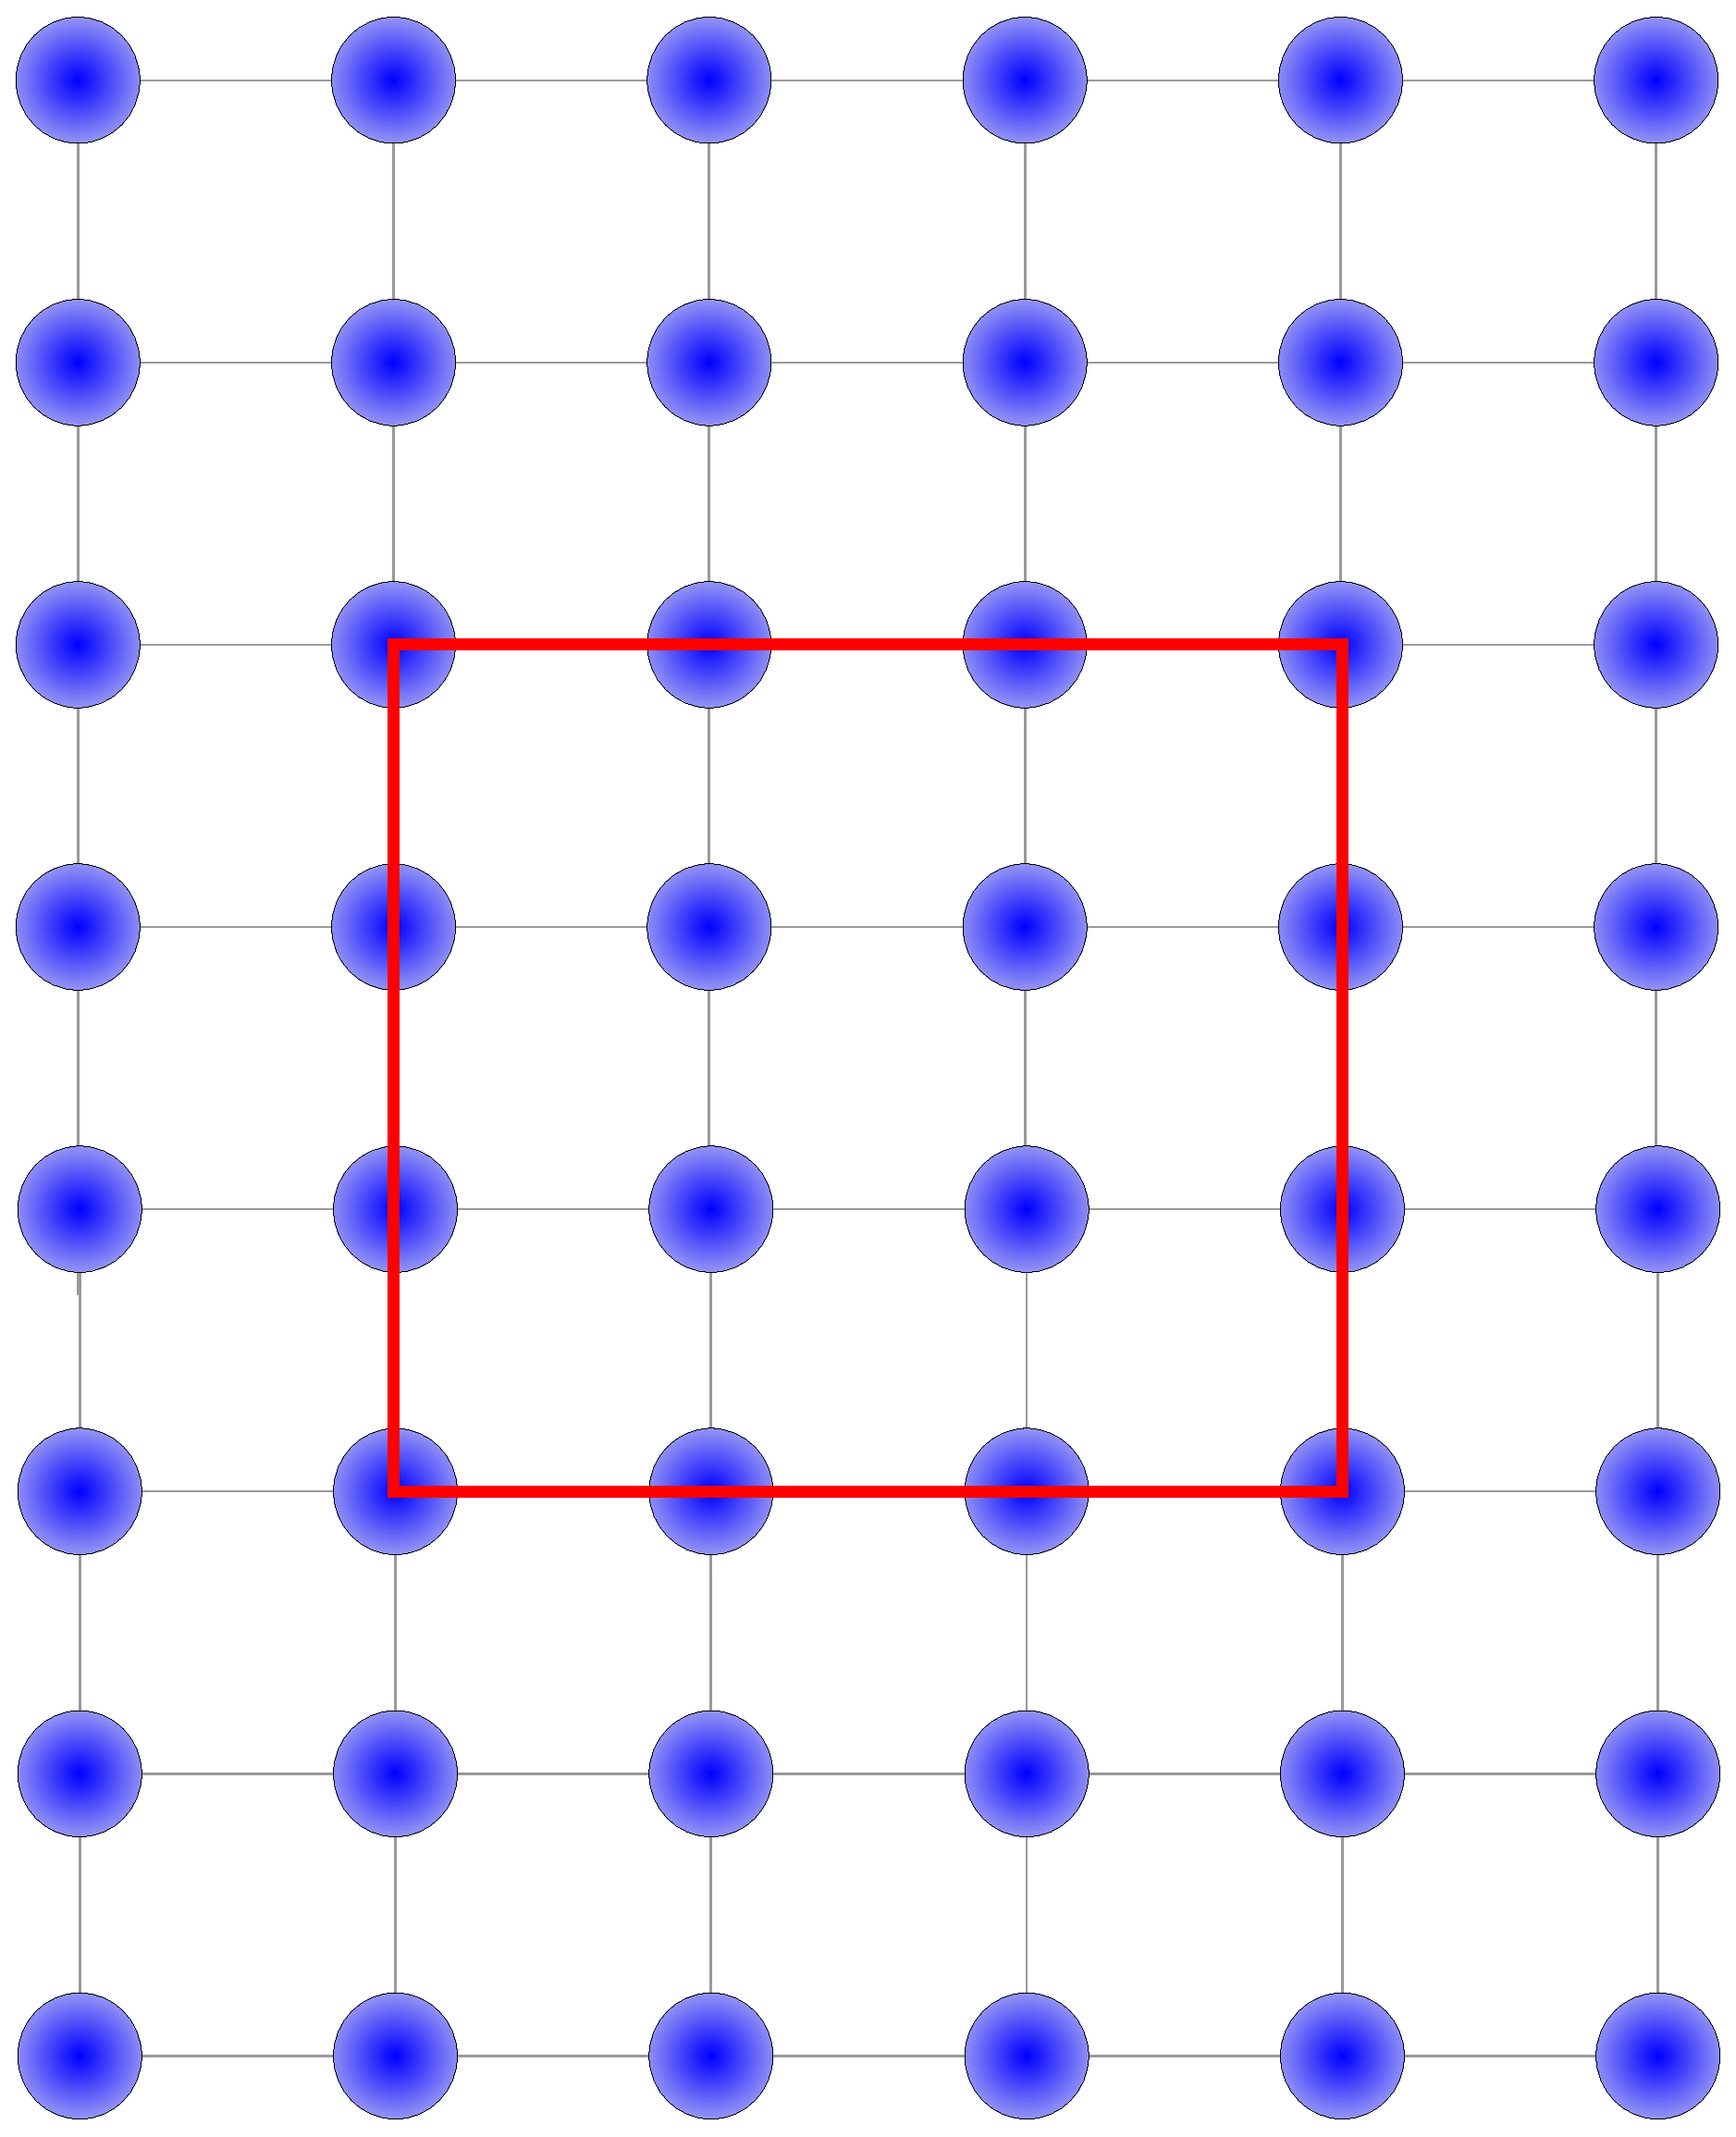
\includegraphics[height=2.5in]{Perfect_crystal_loop}
\caption{A perfect crystal with a complete circuit shown in red.}
\end{subfigure}
\begin{subfigure}{0.4\textwidth}
\centering
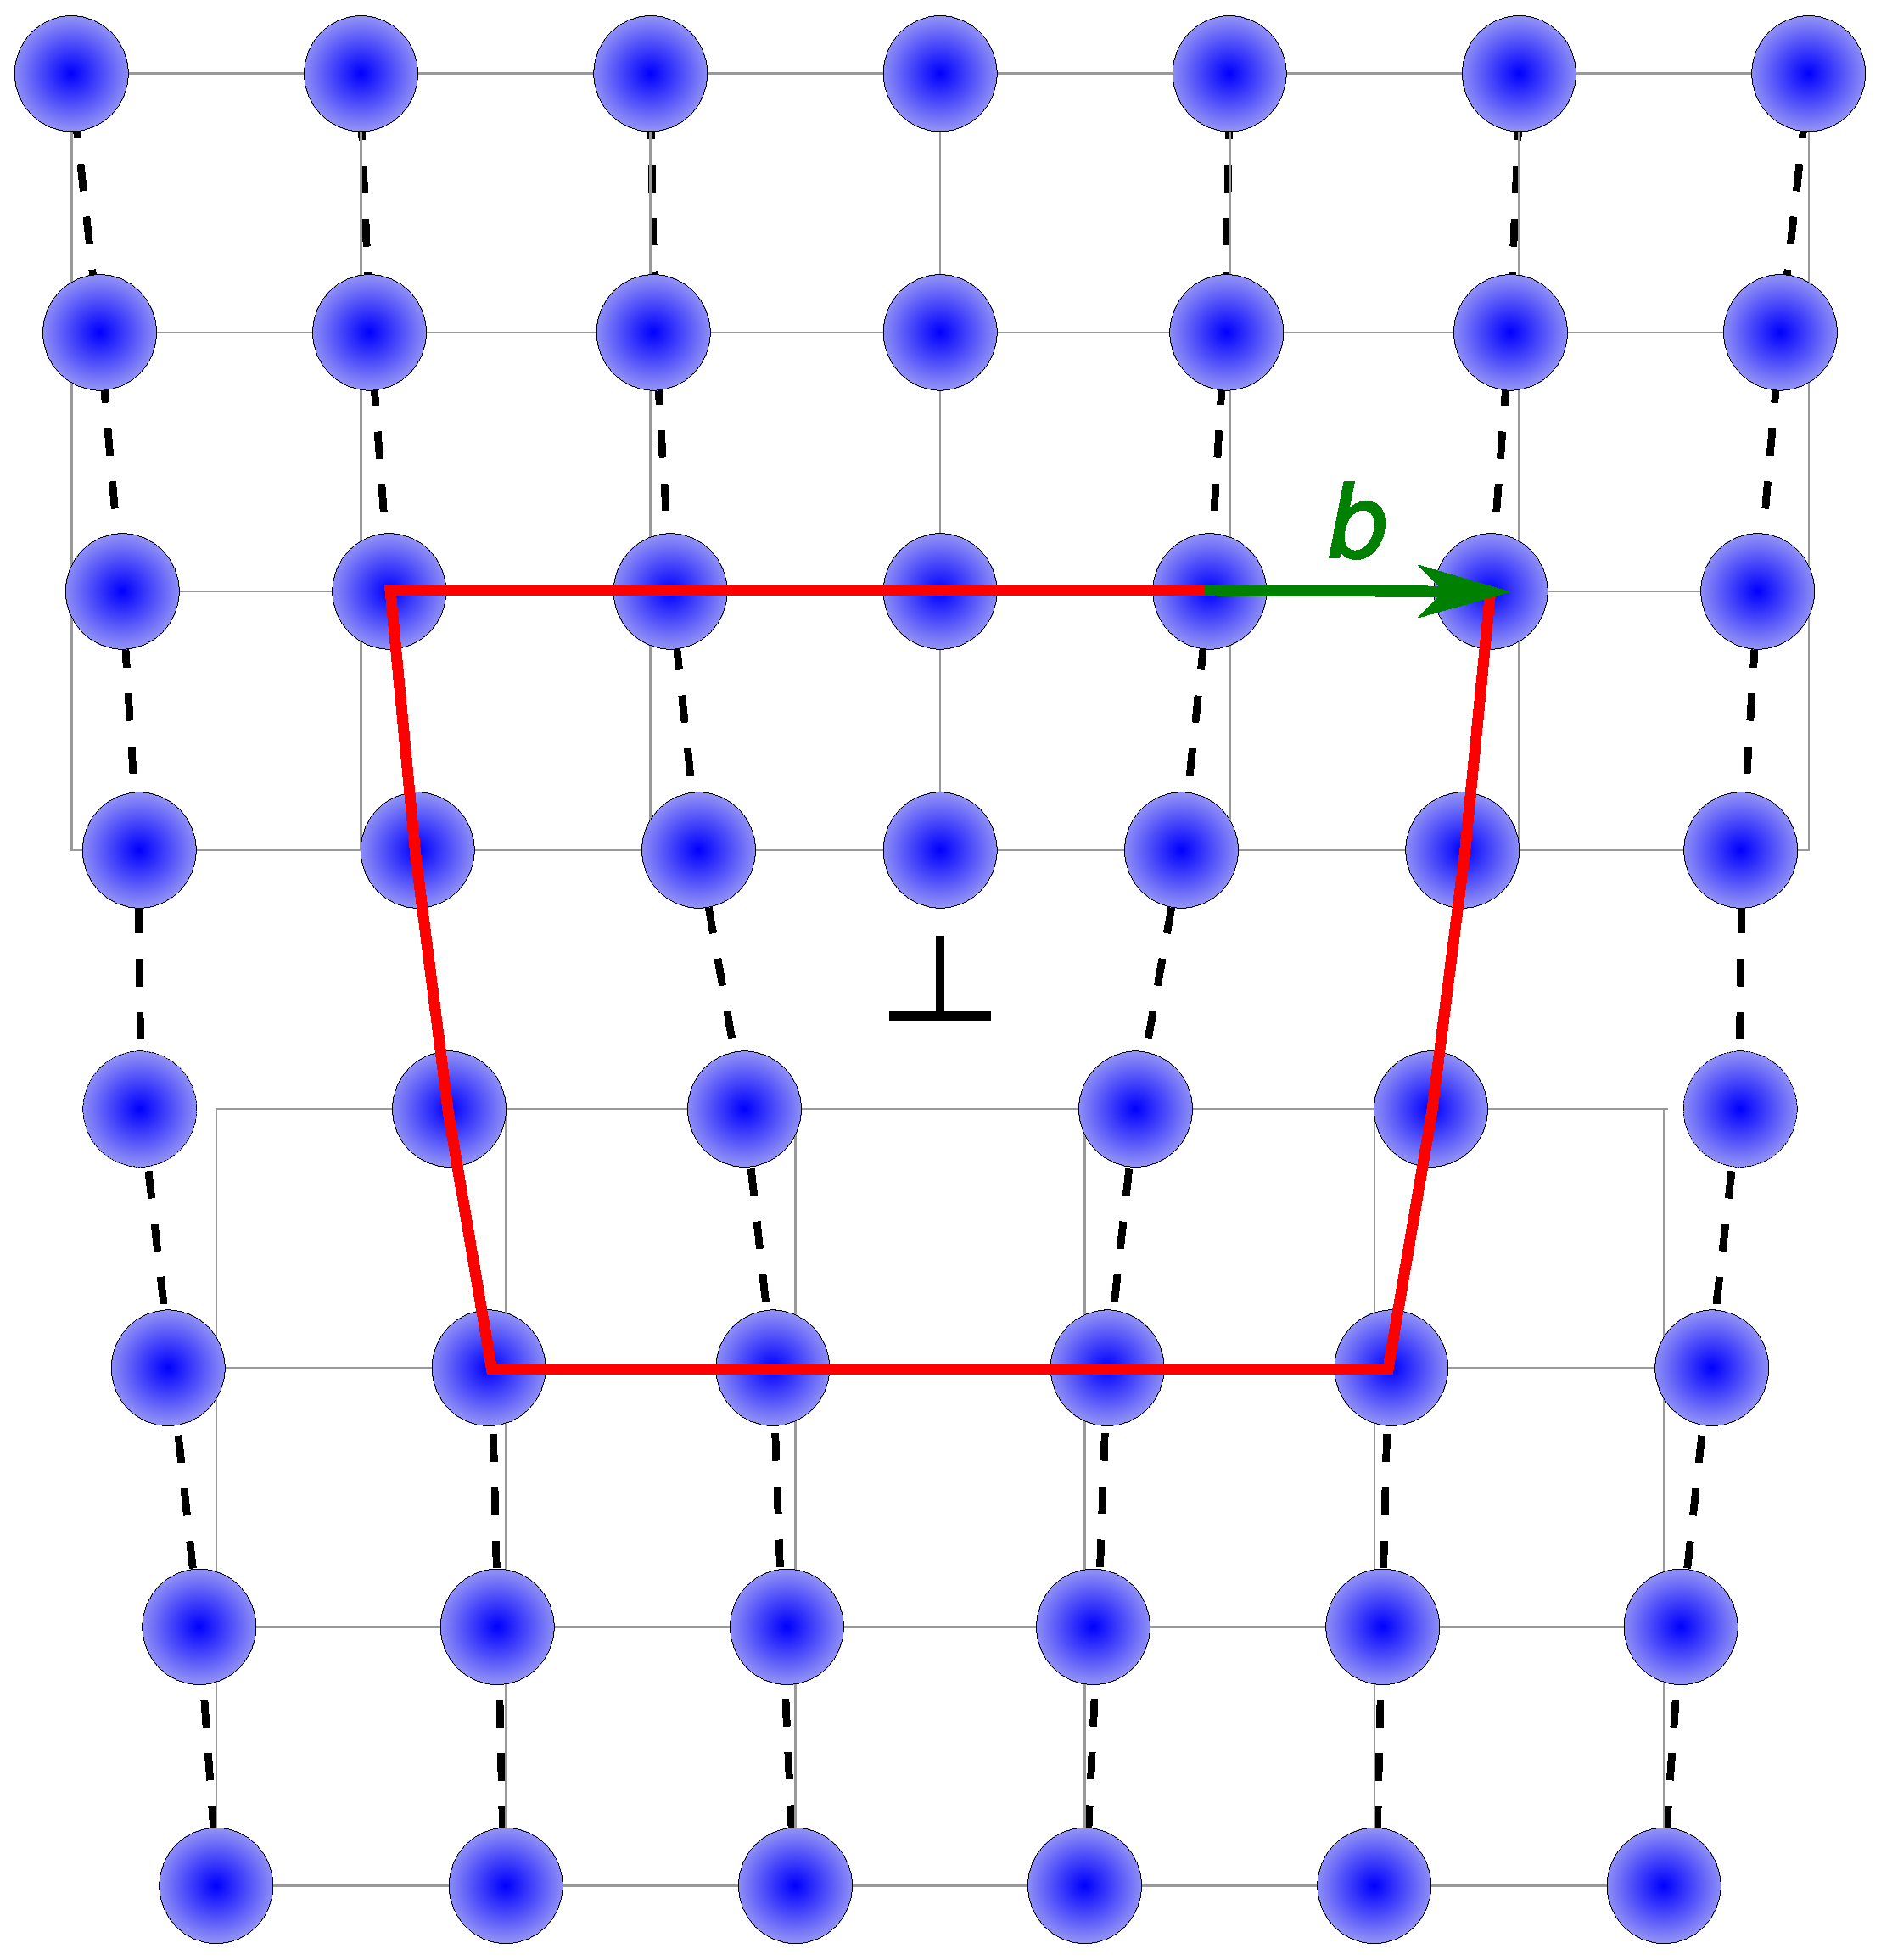
\includegraphics[height=2.5in]{Edge_Dislocation_loop}
\caption{An edge dislocation with an incomplete circuit. \label{fig:Edge_disloc_loop}}
\end{subfigure}

\caption{Inserting a half plane of atoms which terminate in a dislocation and a Burgers circuit to show the Burgers vector. \label{fig:burgers_loops}}

\end{figure}

\begin{figure}
\centering
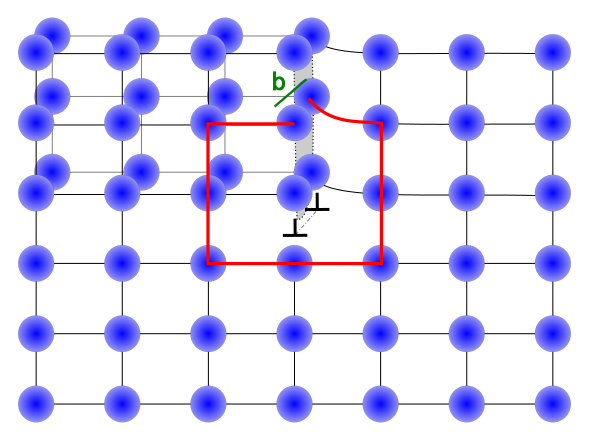
\includegraphics[width=0.7\textwidth]{screw_disloc_loop}
\caption{Schematic of a screw dislocation with a Burgers loop formed in a similar way to \autoref{fig:burgers_loops}. The displacement is parallel to the dislocation line in contrast with edge dislocations. The atomic positions are not relaxed, the displacements being concentrated unphysically into one half plane. \label{fig:screw_disloc}}
\end{figure}




Dislocations can be described in terms of a slip direction, a line direction and a slip plane. The slip direction is simply the direction parallel to the Burgers vector, this is the relative displacement caused by the passage of a dislocation through a region of crystal. The identification of the Burgers vector is done with a Burgers loop, a loop comprised of steps between nearest neighbours is defined that would be closed in a perfect crystal is defined. The same set of steps is undertaken in a dislocated crystal and the loop is no longer closed and the displacement vector between the endpoints is the Burgers vector. This is shown for an edge dislocation in \autoref{fig:burgers_loops}, where the Burgers vector is perpendicular to the line vector, and a screw dislocation in \autoref{fig:screw_disloc}, where the Burgers vector is parallel to the line vector. The line direction can and does vary along the length of the dislocation but is simply the line defined by the defective region of crystal. The slip plane is the crystallographic plane in which the dislocation can move and must contain the slip direction and line direction; where the line and the slip directions are not parallel the slip plane is defined by these two vectors, but for screw dislocations which have the slip direction and line directions parallel the plane is not so constrained, instead the possible slip planes are those that allow easy movement, i.e. lower forces or smaller energy changes, and depending on the crystal symmetry there may be several. This allows screw dislocations to change the plane they are moving in, a process known as cross slip \cite{Hirth_Lothe1982intro}.

Real dislocations are not neat and instead of lining up with convenient crystallographic axes will curve and bend. This usually gives rise to a mixed and varying character of dislocation with the Burgers vector neither parallel nor perpendicular to the line vector. These mixed dislocations are usually described as the sum of edge and screw components.

There are conventions about the sign of dislocations, taking line vectors into or out of the page and defining the sense of Burgers loops and the Burgers vector defined from the finish to the start etc. Given that the symmetry of most of the crystals of interest is high enough to ensure that all these choices are usually arbitrary the only thing that will be highlighted here is that if the sense of a dislocation is reversed then its stress/strain field will reverse in sign. Hence oppositely signed dislocations attract to lower the stored elastic energy and potentially to annihilate line length, while like-signed dislocations will repel to lower the elastic stored energy.



\FloatBarrier

\subsection{Historical overview}


In the early twentieth century there were many observations of real world materials strengths that could not be reconciled with the theoretical shearing strength of a perfect plane of atoms. Indeed for a long time this was neglected because, as \citet{gordon1991} puts it:
\begin{quote}
``Until about 1934 the Establishment explanation of these phenomena was remarkably unconvincing and seems to have reflected mainly a desire not to be asked embarrassing questions.''
\end{quote}

In 1934 the edge dislocation was proposed by \cite{orowan1934i,Orowan1934ii,Orowan1934iii}, \citet{Taylor1934}, and \citet{polanyi1934} to explain the discrepancy between the ideal strength of crystal and the observed strengths of real materials. It was around this time that work undertaken by \citet{Volterra1907} and others, particularly \citet{love1920}
on elastic behaviour of homogeneous isotropic continua was related to plastic flow of crystalline materials, idealised dislocations in elastic continua are termed Volterra dislocations. By the end of the decade \citet{burgers1939} had described screw dislocations. 

It was not until the 1950s that experimental evidence for the existence of dislocations was produced; the initial evidence was growth surfaces of single crystals, preferential etching of a crystalline material at dislocations and x-ray studies of arrays of dislocations in the bulk \cite{Forty1954}. 

\citet{Frank1949} predicted, in 1949, that a step could terminate by the intersection of a dislocation with a free surface, or conversely a dislocation intersecting with a free surface would necessarily create a step; these weere observed soon after in 1950 by \citet{Griffin1950}. Preferenctial etching of dislocations was observed by \citet{horn1952holes} who matched the configuration of etch pits with the pre-existing surface growth features that arise from screw dislocations. The effect of plastic work and subsequent recovery on Laue spots (the xray beams diffracted by a single crystal) provide evidence of arrays of dislocations. The process is described by \citet{Cottrell1949}: Initially sharp Laue spots exist in a perfect crystal. Plastic work smears the spots by introducing a homogeneous distribution of dislocations and the spots then split into distinct sharp spots during recovery as dislocations align into arrays that form sub-grains with small misalignments across the new low angle grain boundaries.


An edge dislocation was first imaged in 1956 by \citet{Menter1956} in platinum phthalocyanine. The large organic complex with a platinum atom at the centre produces widely spaced rows of platinum atoms suitable for imaging with transmission electron microscopy.




\subsection{The stress required to move a dislocation}

Though mathematical descriptions of dislocations in isotropic elastic continua date back to 1907 \cite{Volterra1907} the energies and forces around dislocations in crystalline lattices and the  was not considered until much later. In 1940 \citet{Dehlinger1940} and \citet{Peierls1940}. The former presented the application of the Frenkel-Kontorova model, a one dimensional array of balls connected by springs on a periodic potential/substrate, to approximate a dislocation.

The latter, Rudolph Peierls, was one of the physicists working during the advent of quantum mechanics and most of his work was in that field, however during his education he received a grounding in classical physics at Arnold Sommerfeld's lectures in Munich and so it was that he was suitably equipped when presented with the problem of dislocation motion by Egon Orowan; as Peierls remarked he knew nothing about dislocations but he did know classical elasticity \cite{Edwards1996}.


Peierls presented the first formal solution for the energy changes as a dislocation moves in a rather short note \cite{Peierls1940} and the idea was extended by \citet{Nabarro1947}. The model is remarkably simple; consider two semi-infinite perfect crystals with their lattice aligned but some initial misalignment between them as shown in \autoref{fig:semi_infinite_crystals}. We can join them along what will become the slip plane. An edge dislocation is formed where the energy of the system is lowered by displacing atoms from their initial positions to localise the misalignments around the dislocation core, usually taken to be the origin. I.e. when the energy of a planar defect is higher than that of the linear defect and dislocation will form.



\begin{figure}
\centering

    \begin{subfigure}{0.4\textwidth}
        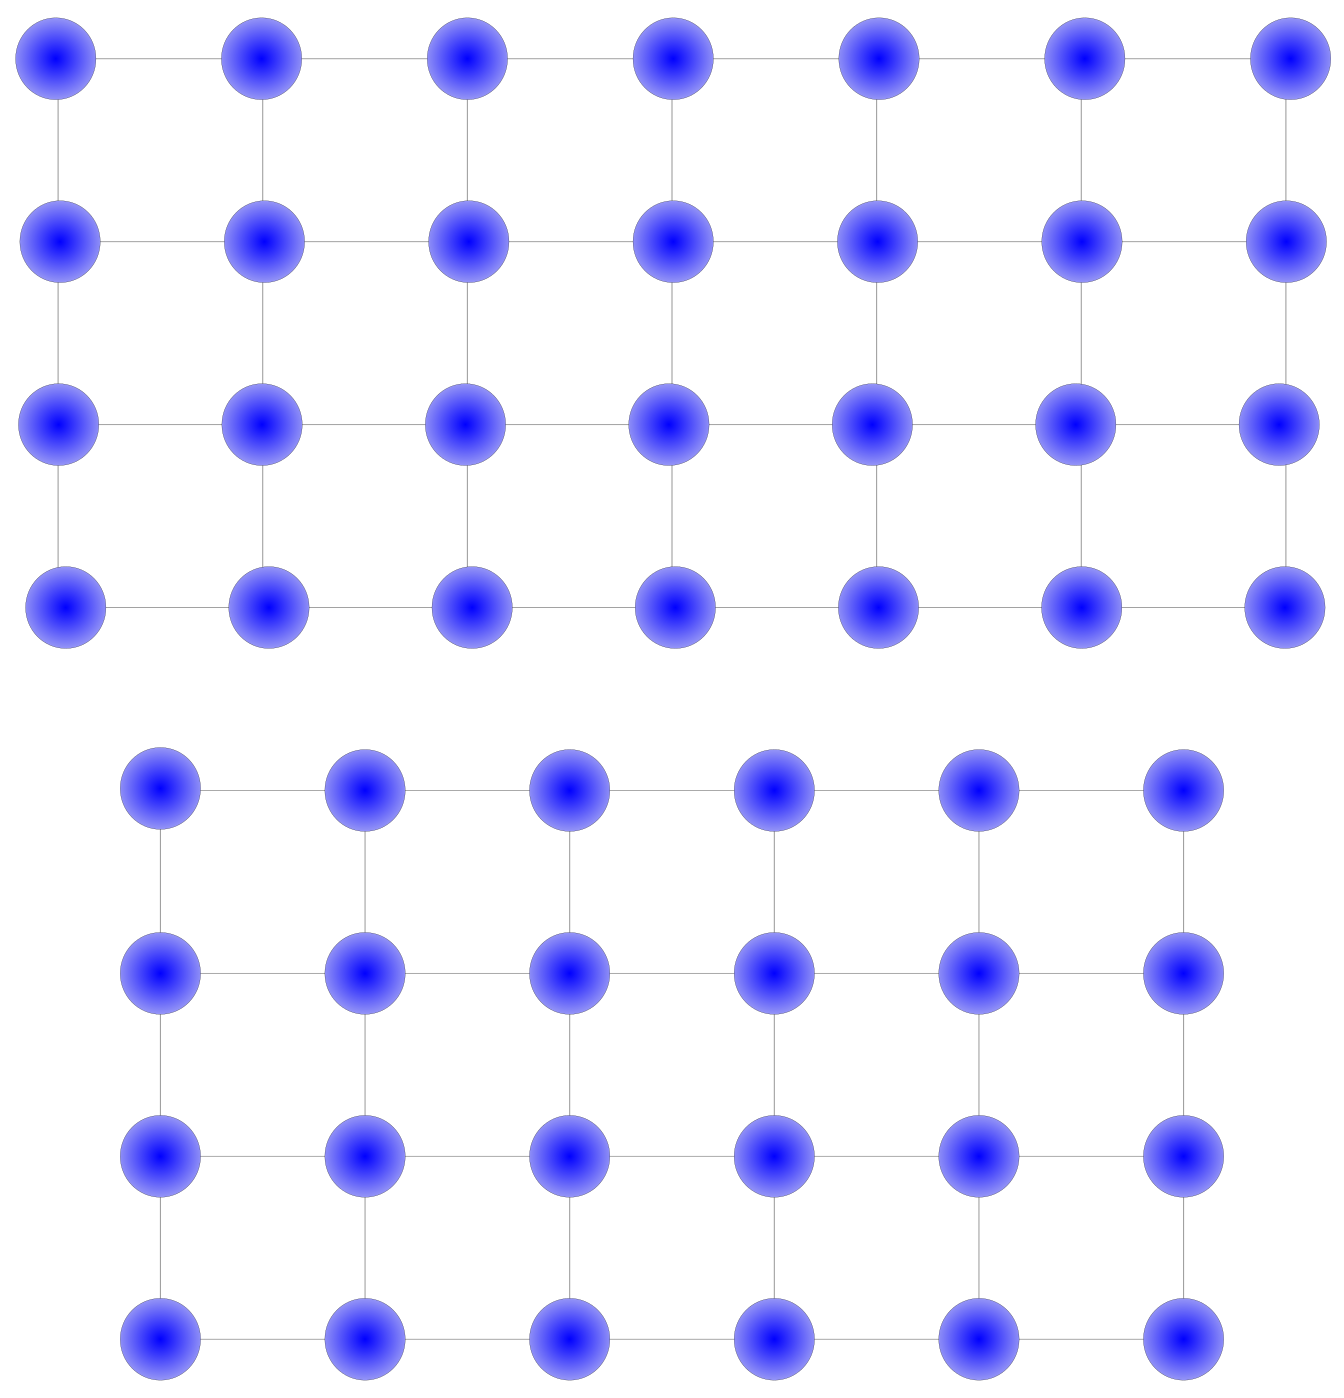
\includegraphics[width=\textwidth]{Half_crystals}
        \caption{Two semi-infinite crystals \label{fig:semi_infinite_crystals}}
    \end{subfigure}

    \begin{subfigure}{0.4\textwidth}
        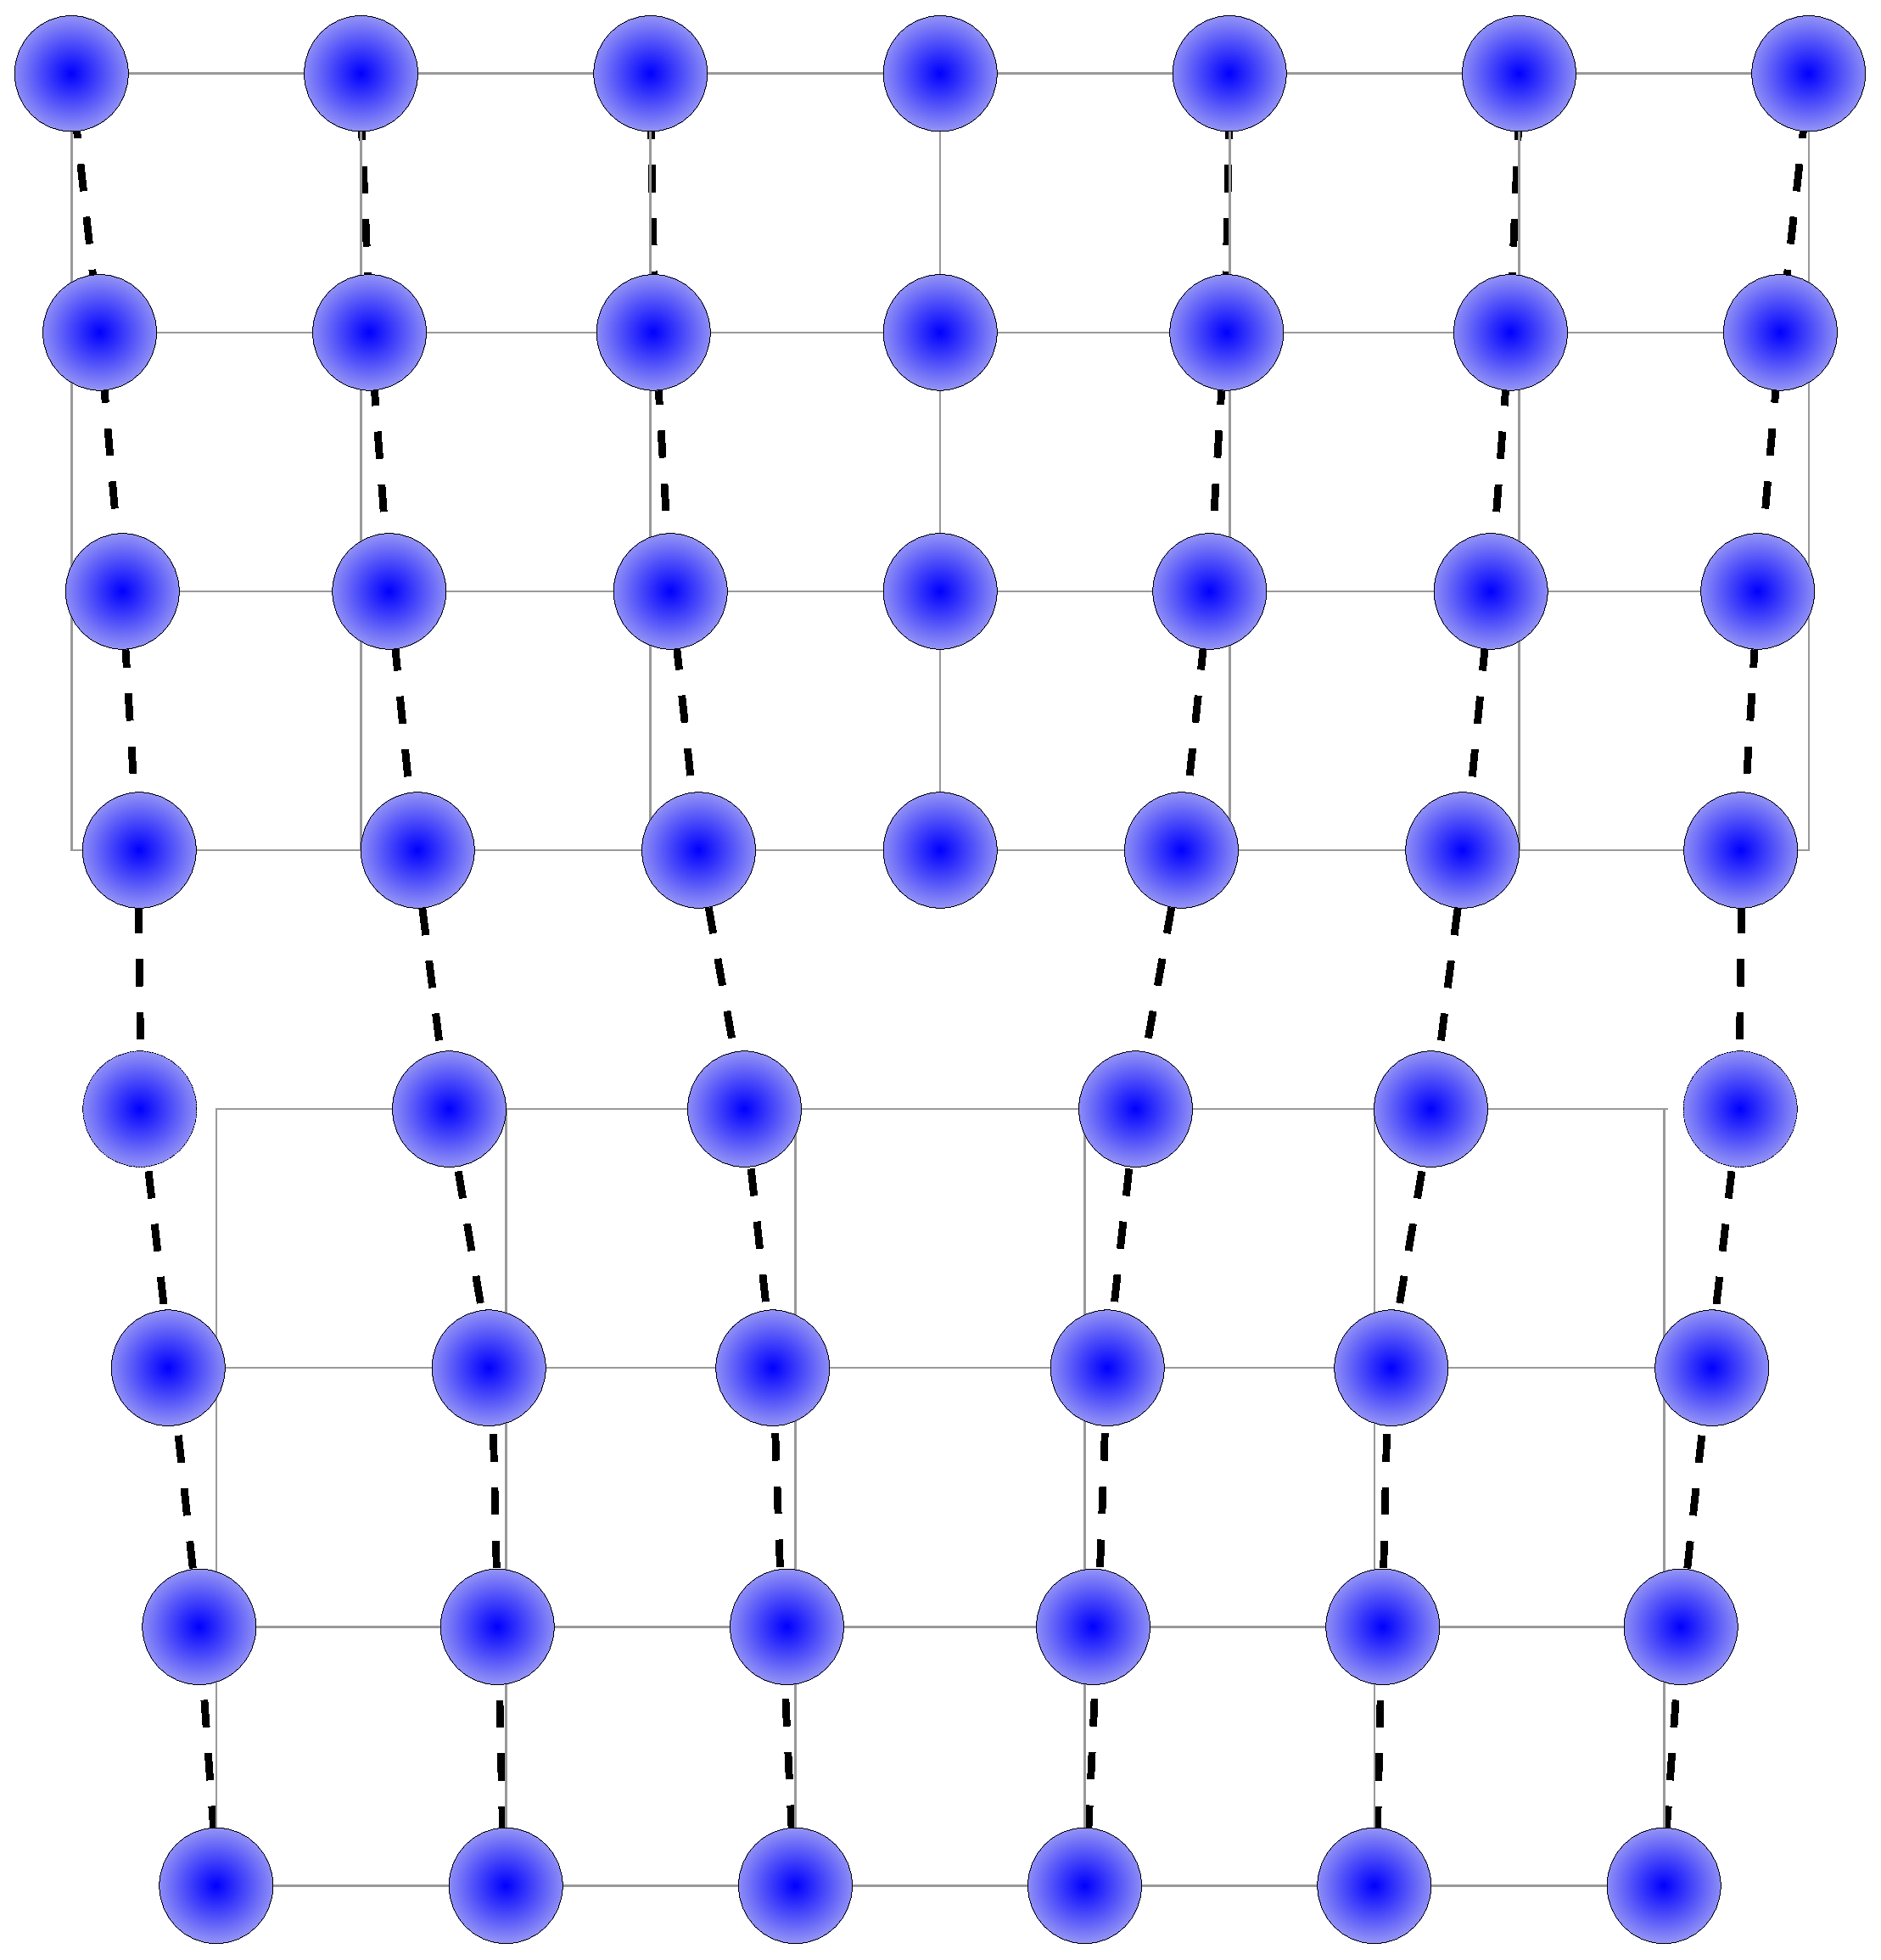
\includegraphics[width=\textwidth]{Edge_Dislocation}
        \caption{A schematic edge dislocation\label{fig:joined_half_crystals}}
    \end{subfigure}

    \caption{Schematics showing the creation of an edge dislocation in a simple square lattice by the joining of two misaligned half crystals. \label{fig:edge_disloc}}
\end{figure}

\begin{figure}
\centering
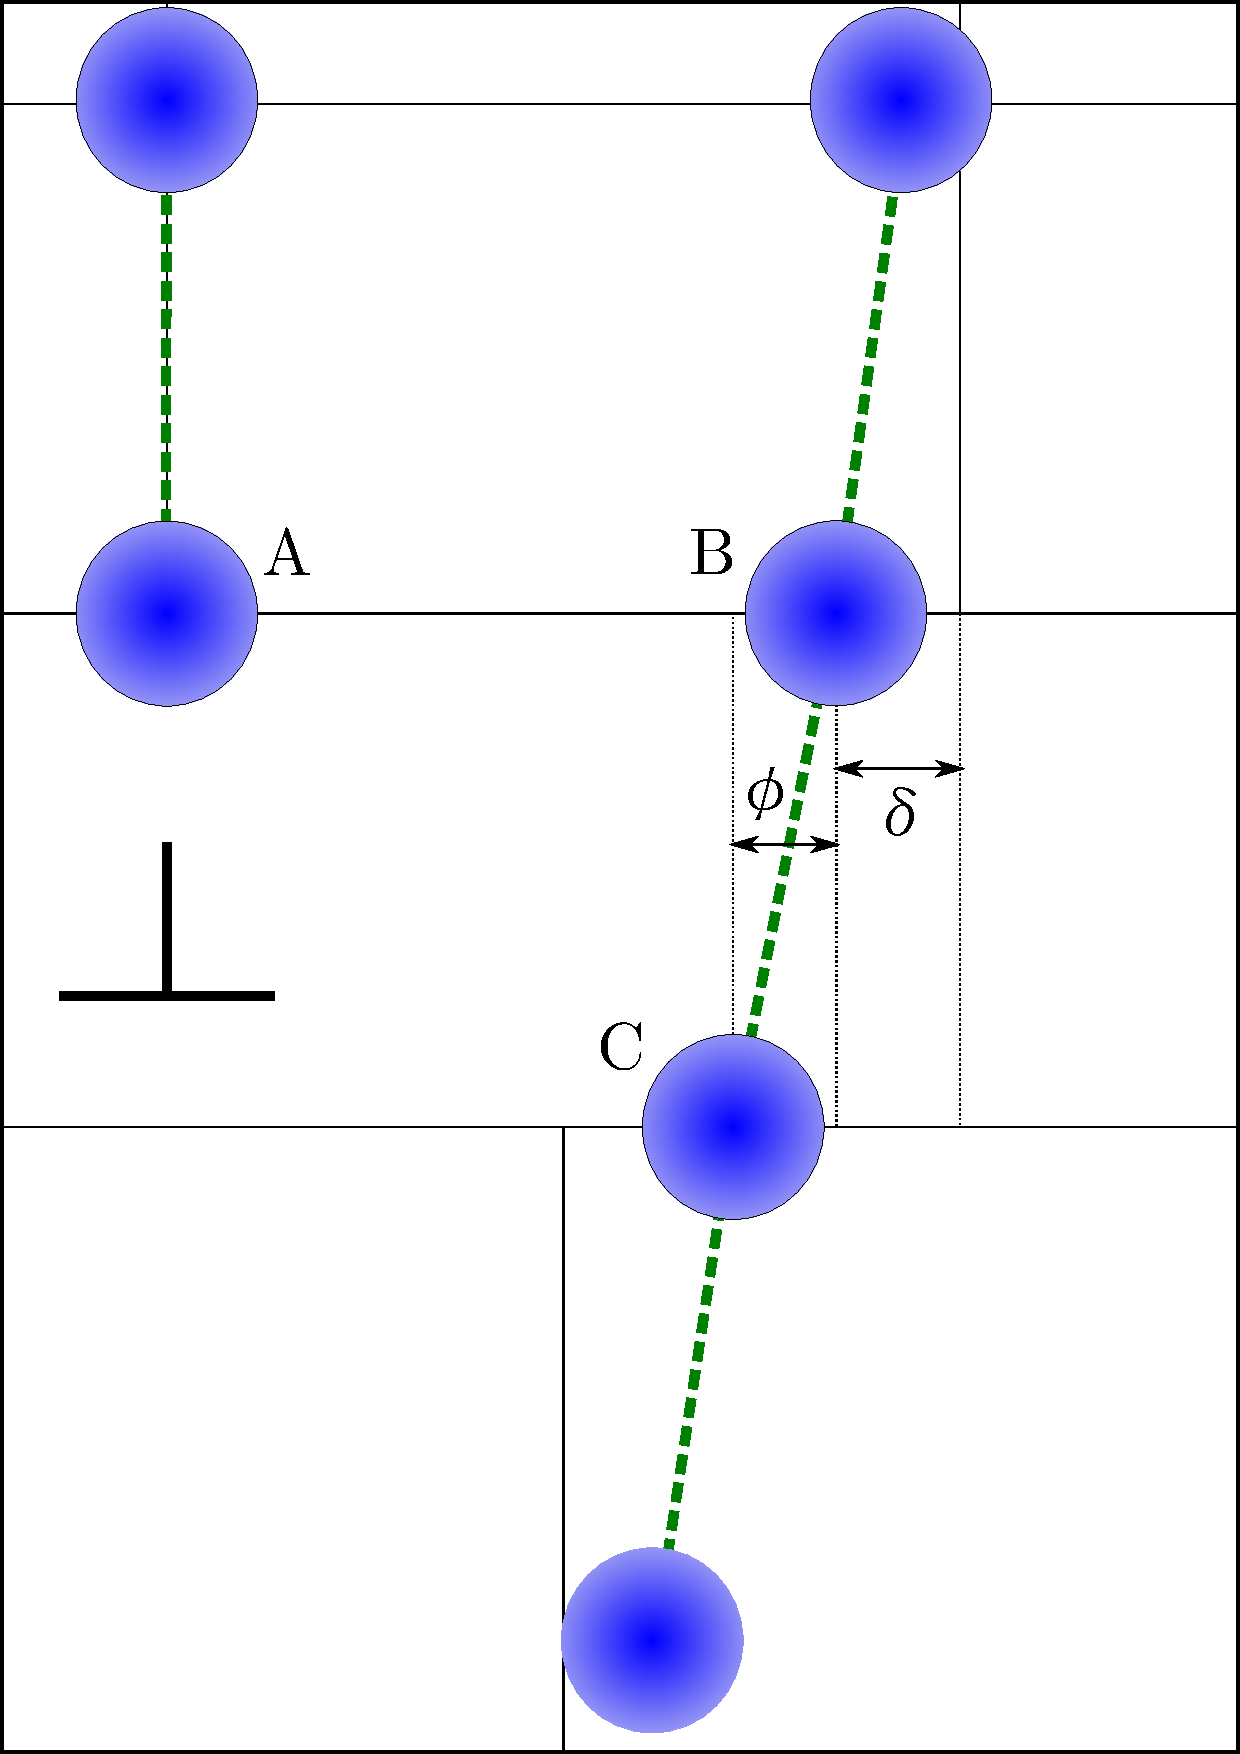
\includegraphics[width=0.6\textwidth]{peierls_model_detail}

\caption{Detail of the local displacements around the dislocation core. $\delta$ is the extension of the bond parallel to the slip plane between atoms A and B, while $\phi$ is the misalignment of the bond across the slip plane between B and C.\label{fig:detail_of_peierls}}
\end{figure}

Atomic configurations that form a dislocation are generated by by applying a displacement field to the atoms immediately above and below the slip plane, $u(x)$ and $u'(x)$ respectively. The Peierls model then estimates the energy of the configuration by considering two restoring forces generated by the atomic arrangement. The detail is show in \autoref{fig:detail_of_peierls}. Firstly the bonds parallel the slip plane will be either extended or contracted, for example the bond between atom $A$ and $B$ has been contracted by the amount $\delta$, this will tend to oppose the concentration of misalignments to the core and is zero in the case of no displacements from the initial positions. Secondly the misalignment of bonds across the slip plane, the bond between atom $B$ and $C$ is misaligned by a lateral distance of $\phi$. This misalignment energy will tend to favour the concentration of the misalignments to the core and is a maximum in the case of no displacement from the initial position.

Peierls made the assumption that the displacements vary slowly with position, i.e. that the dislocation is very wide. This means that the strain in the slip plane (i.e bonds like $\overrightarrow{AB}$ in \autoref{fig:detail_of_peierls}) experience only small strains. The energy associated with these \emph{in-plane} strains are then described  by the application of the displacement field to the surface of two semi infinite elastic continua. 
The \emph{misalignment} energy of bonds across the slip plane (bonds like $\overrightarrow{BC}$ in \autoref{fig:detail_of_peierls}) is assumed to be a periodic function, specifically a simple sinusoidal variation is taken to be the form of the misalignment potential:

\begin{equation}
U_{mis} = C \sin \left(\frac{2\pi [u(x) - u'(x)]}{d} \right)
\end{equation}













%%%%%%%%%%%%%%%%%%%%%%%%%%%%%%%%%%%%%%%%%%%%%%%%%%%%%%%%%%%%%%%%%%%%%%%%%%%%%%%%%%%%%%


%
%
%
%
%   Sort out this Frenkel stuff
%
%
%
%
%
%


%%%%%%%%%%%%%%%%%%%%%%%%%%%%%%%%%%%%%%%%%%%%%%%%%%%%%%%%%%%%%%%%%%%%%%%%%%%%%%%%%%%%%%



The constant, $C$, has to be chosen appropriately but can be found by assuming linear elasticity holds at small strains. \citet{Frenkel1926} derived a similar sinusoidal function for the stress to form a stacking fault:










\begin{equation}
\tau_{fault} = \tau_{\text{theory}} \sin \left( \frac{2\pi \phi}{b} \right)
\end{equation}

The energy of the dislocation is the sum of all these contributions. There will be a configuration that is a minimum in the total energy where the in-plane forces widening the dislocation balance the misalignment forces that drive it to be narrower. This gives rise to a size, or width, of a dislocation. The width of the dislocation is defined as the distance from the core at which the misalignment across the slip plane is half its maximum. Peierls calculated this for an isotropic elastic solid and accounting for only the atomic planes immediately adjacent to the slip plane and found it to be 

\begin{equation}
w = \frac{d}{1-\nu}
\label{eqn:width_isotropic}
\end{equation}
where $d$ is the plane spacing across the slip plane and $\nu$ is the Poisson ratio.

The stress required to move a dislocation can be calculated from the maximum energy \emph{gradient} as the dislocation is displaced. Since the in-plane strains have a continuous definition in this model the displacement of the dislocation has no effect and the in-plane strain energy does not change. The energy changes therefore depend only on the misalignment energy of bonds across the slip plane and the energy of all the atoms away from the slip plane re neglected.

Peierls gave the critical stress, the \emph{Peierls Stress}, for an isotropic elastic material in terms of the ideal shear strength as calculated for uniform slip and accounting for only the interactions between the first plane either side of the slip plane, as


\begin{equation}
\frac{\tau_p}{\tau_{ideal}} = \frac{4 \pi}{1 - \nu} (5.8 - \log|1-\nu|) \exp\left(-\frac{4\pi}{1 - \nu}\right).
\end{equation}

This was refined by \citet{Nabarro1947} and the direct summation of the discrete contributions was developed by Cottrell and Nabarro \cite{Cottrell1953}. The result of that summation is



\begin{equation}
\tau_p = \frac{2\mu}{1-\nu} \exp\left( - \frac{4\pi w}{b} \right)
\end{equation}
where $\mu$ is the shear modulus and $b$ is the burgers vector.

For an isotropic material the width can be substituted from \autoref{eqn:width_isotropic}:

\begin{equation}
\tau_p = \frac{2\mu}{1-\nu} \exp\left( - \frac{2\pi d}{(1-\nu)b} \right).
\end{equation}

Although this simple model includes some large assumptions the method moved dislocation theory on in two ways: firstly continuum elasticity could not account for energy changes as the dislocation moves since in an isotropic homogeneous continuum one dislocation position is identical to all others and there will be no energy changes as the dislocation move, and secondly this approach removes the singularity at the core predicted by continuum elasticity for Volterra dislocations.


An important point to note is that the Peierls stress is extremely sensitive to the size of the dislocation, $w$, and therefore to the factors that control the width; which in turn is defined by the lattice geometry, $d/b$, and the elastic properties.



Peierls found the perhaps surprising result that the energy changes have a periodicity of $b/2$ rather than $b$, this has been ascribed to the summation procedure of the energy of the misaligned bonds across the slip plane, of which there has been much discussion \cite{Hirth_Lothe1982lattice_periodicity,Lu2000peierls}. Peierls summed over the atoms above the slip plane and below the slip plane independently, the ``double-counting'' scheme, later models used a ``single-counting' scheme in which the assumption of small displacements is dropped and the misalignment of an atom above the slip plane is dependent on the final position of the atoms below the slip plane. This is given as the reason the Peierls barrier had a wavelength of $b/2$ rather than $b$ \cite{Hirth_Lothe1982lattice_periodicity,Lu2000peierls} though it has been suggested that the problem is an artefact that arises from an assumption of small displacements and that using the final rather than initial positions of the atomic rows resolves the difficulties \cite{Huntington1955}. There is another explanation for the change in period that depends on the exact formulation of the energy calculations and whether the $\alpha=1/2$ position is symmetrically equivalent to the $\alpha = 0, 1$ positions. The periodicity of $b/2$ is easily explained on this basis because Peierls assumed that both the elastic energy and the dislocation geometry remained constant and the only changes in the energy were therefore based on misaligned bonds across the slip plane. These assumptions produce an atomic configuration at $\alpha=1/2$ that is the a reflection  of the $\alpha=0$ configuration across the slip plane, which must give the same energy since the misalignment potential used by Peierls is symmetrical.




There have been many criticisms of and modifications to the Peierls model in the years since but these have largely focused on adjusting the assumptions of the original method.
In 1951 \citet{Foreman1951} introduced phenomenological potentials to describe the energy of the misaligned interactions across the slip plane, they discovered that the width of the dislocation was predicted to be larger than that of the original treatment and was coupled with a decrease in the Peierls stress.

In 1955 \citet{Huntington1955} modified the model to double the periodicity and so account for crystals in which a displacement of half a burgers vector is not symmetrical with no displacement, or in other words broke the mirror symmetry of the slip plane. 
\citet{Maradudin1959} considered a completely atomistic three dimensional model of a screw dislocation but did not consider radial displacements. That work only evaluated the energies of the symmetric and anti-symmetric configurations and so only estimated the energy change, not the maximum stress.



In 1994 a fully discrete model was developed by \citet{Ohsawa1994}. This model made similar assumption to the original Peierls model in that the only energy changes were in the sheared misaligned bonds across the slip plane but instead of solving for an analytical solution Ohsawa et al. used numerical methods to optimise the configuration of 84 atoms,  either side of the dislocation core. The model made no assumptions about the displacement field and instead iteratively improved all the atomic positions to find the equilibrium configuration. This was done for increasing applied external stresses until there was no stable configuration, at which point slip would occur.





The generalised stacking fault (GSF) energy or $\gamma$-surface was incorporated into the Peierls model by \citet{Vitek1992} and this was extended by \citet{Bulatov1997}. This addresses a fault in the original Peierls formulation that the sinusoidal potential used to calculate the misalignment energy is too high and steep. \citet{Ohsawa1994} had already attempted to address this by using alternative potentials, but they were essentially arbitrary functions that fitted the shear modulus at small strains instead Bulatov et al. retained the variational approach but used density functional theory (DFT) calculations to generate a misalignment potential, extending the model to include a three dimensional potential to allow both lateral and vertical displacements of the atoms in the slip plane. This is important around the core where large strains mean that the energy contributions are very inaccurate. By using the DFT to calculate the misalignment potential the Peierls model can bridge the length scales between the large scale stress and strain fields around the dislocation and the large local displacements at the core. This is no longer analytically solvable but is not difficult to solve numerically, the only limit being computational time.

Analytical approaches have continued, \citet{Joos1997} developed a closed form solution that was valid for narrow dislocations, where as the original model relied on the assumption of a wide dislocation for simplicity, and achieved a significantly better agreement with experiment than the original formulation. The model proposed by Joós and Duesbery required input parameters calculated by empirical or ab initio methods but used these as parameters of a closed form solution, in particular they required the maximum restoring stress for the glide plane, i.e. the maximum gradient of the GSF energy.

\begin{figure}
\centering
\begin{subfigure}{0.4\textwidth}
\centering
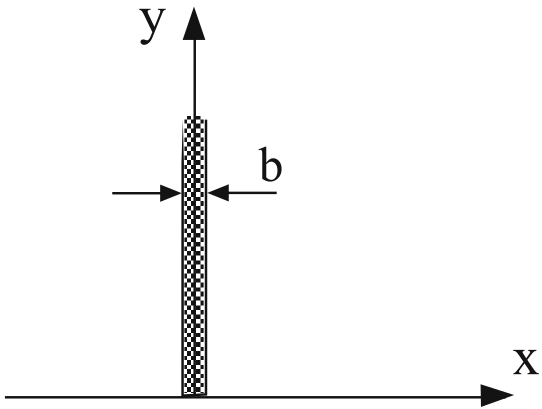
\includegraphics[width=0.75\linewidth]{Dislocation_with_discontinuity}
\caption{Volterra dislocation.\label{fig:disloc_discontinuity}}
\end{subfigure}%
\begin{subfigure}{0.4\textwidth}
\centering
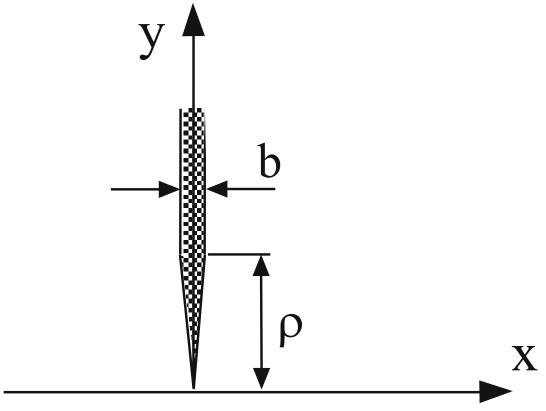
\includegraphics[width=0.75\linewidth]{Dislocation_without_discontinuity}
\caption{Lubarda dislocation\label{fig:disloc_no_discontinuity}}
\end{subfigure}
\caption{The displacement discontinuities in the traditional Volterra dislocation and that used by Lubarda and Markenscoff that removes the singularity at the core. From \cite{Lubarda2007}\label{fig:discontinuity}}
\end{figure}

A continuum elasticity solution was presented by \citet{Lubarda2007} which removed some of the limiting assumption of the original Peierls model, notably the assumption of fixed dislocation geometry as the dislocation was translated from one symmetrical position to the next and that only the misfit energy of the slip plane changes and that the elastic energy away from the slip plane remains constant. The main challenge to using continuum elasticity to solve the Peierls model directly is the singularity in stress and strain at the dislocation core. 
This singularity arises where the displacement discontinuity of a Volterra dislocation across the half plane of an edge dislocation terminates at the core shown in \autoref{fig:disloc_discontinuity}. 
By introducing a gradual increase in the displacement discontinuity across the plane of an edge dislocation from zero at the core to $b$ at some finite distance, as shown in \ref{fig:disloc_no_discontinuity}, Lubarda and Markenscoff were able to formulate a tractable linear elastic continuum problem which produced much better agreement than previous analytical solutions. They found this distance to be be interpretable as the width of the dislocation giving rise to displacements that are consistent with the original Peierls model. 



In 2006 \citet{Clegg2006} used an atomistic approach to the strains outside of the slip plane in addition to the energy of the misalignment across the slip plane. The atomic displacements were taken to have the same form as Peierls had derived, that is

\begin{equation}
u(x_0) = \pm \tan^{-1}\frac{x_0}{w}.
\end{equation}

where $x_0$ is the initial coordinate in the dimension parallel to the burgers vector and $w$ is the dislocation width, now a parameter to be optimised with no closed form solution. The misalignment energy was taken to be

\begin{equation}
U^{x} = \frac{Gb^3}{4\pi^2 d} \sum_n \left[ 1 - \cos \left(\frac{2\pi \phi_n}{d} \right)\right]
\end{equation}
 
 and the in-plane strain energy was taken to be 
 
 \begin{equation}
 U^i = \frac{E}{2(1-\nu^2)} (b\cdot d) \sum_n \epsilon_n^2
 \end{equation}

where $G$ is the shear modulus of the material, $E$ is the Young's modulus, $\nu$ is the Poisson ratio, $b$ is the Burgers vector, $d$ is the slip plane spacing, $\epsilon$ is the strain and is calculated by $\epsilon = \delta/b$, $\delta$ is the extension of an in plane bond and $\phi$ is the misalignment of the bond across the slip plane. $\phi$ and $\delta$ are shown in \autoref{fig:detail_of_peierls}. The energies are then summed over interaction between atomic rows extending 1000 atomic spacings either side of the dislocation core.

The width no longer has an analytical solution so must be found numerically. The variation of the energy was shown to be smooth and have only one minimum because the misalignment energy is monotonically increasing with increasing width and the elastic in plane strain energy is monotonically decreasing.

It is interesting to note that this formulation restores the symmetry that is destroyed in the calculation of elastic energy by continuum elasticity in that the strains above and below the slip plane are symmetric. So despite allowing the strain energy to vary as the dislocation moves this model has the same period as the original Peierls model of $b/2$.


